\documentclass[conference]{IEEEtran}
\usepackage{cite}
\usepackage{amsmath,amssymb,amsfonts}
\usepackage{algorithmic}
\usepackage{graphicx}
\usepackage{textcomp}
\usepackage{xcolor}
\usepackage{booktabs}
\usepackage{multirow}
\usepackage{hyperref}
\usepackage{float}
\usepackage{subcaption}

\graphicspath{{./figures/}}

\def\BibTeX{{\rm B\kern-.05em{\sc i\kern-.025em b}\kern-.08em
    T\kern-.1667em\lower.7ex\hbox{E}\kern-.125emX}}

\begin{document}

\title{Deep Reinforcement Learning with Specular Reflection Control for Mobile Robot Collision Avoidance Based on Multi-Directional Distance Perception}


\maketitle

\begin{abstract}
Safe autonomous navigation in cluttered environments remains a fundamental challenge for mobile robots. This paper presents a two-stage framework that combines supervised collision prediction with deep reinforcement learning (DRL) for collision avoidance, centered on a physics-inspired specular reflection control mechanism. A Pygame-based 2D simulation environment is constructed, in which a mobile robot is equipped with nine multi-directional range sensors covering a $\pm120^\circ$ field of view. First, a multi-layer perceptron (MLP) is trained to predict future collisions within a 30-frame horizon using 11-dimensional sensor-motion features, achieving an accuracy of 83.65\% and a recall of 84.08\% on held-out test episodes. Second, the collision avoidance problem is formulated as a Markov decision process with a 14-dimensional state space and two discrete actions, where a deep Q-network (DQN) learns \emph{when} to initiate an avoidance maneuver while the \emph{how} is handled by a deterministic three-phase pipeline: deceleration, specular reflection, and re-acceleration. The reflection direction is computed geometrically from the incident heading vector and the obstacle surface normal via $\mathbf{r} = \mathbf{d} - 2(\mathbf{d} \cdot \mathbf{n})\mathbf{n}$. We conduct systematic model iterations across five versions (V1 through V4 and V3-Shield), examining the effects of reflection normal extraction, reward function design, state representation, dynamic braking distance, and external safety intervention. Comprehensive experiments demonstrate that the final V3 DQN policy achieves a collision rate of 1.20\% with a survival rate of 98.80\% over 500 blind-test episodes, substantially outperforming earlier versions and baseline strategies. Notably, our results reveal that increasing model complexity and adding external safety rules do not necessarily improve performance---V4 (17-dimensional state with dynamic braking) and V3-Shield (external safety patch) both exhibit higher collision rates than V3. This finding underscores the importance of maintaining a stable coupling between perception, learned decision-making, and geometric control, rather than adding unvalidated safety heuristics on top of a trained policy.
\end{abstract}

\begin{IEEEkeywords}
collision avoidance, deep reinforcement learning, DQN, specular reflection, robot navigation, collision prediction, multi-sensor perception
\end{IEEEkeywords}

\section{Introduction}

With the rapid advancement of intelligent manufacturing, warehouse logistics, public services, and specialized field operations, mobile robots are increasingly transitioning from structured environments to unstructured settings characterized by random obstacles, complex boundaries, and uncertain disturbances~\cite{siegwart2011introduction}. During autonomous operation, robots must continuously adjust their motion based on limited perceptual information while avoiding collisions with walls, equipment, and other obstacles. Collisions not only disrupt task execution but may also cause equipment damage and pose safety risks. Therefore, accurately identifying potential collision risks and executing timely, effective avoidance maneuvers are critical problems in autonomous robot navigation and safety control.

Traditional approaches to collision avoidance include artificial potential field methods~\cite{khatib1986real}, vector field histograms (VFH)~\cite{borenstein1991vector}, and the dynamic window approach (DWA)~\cite{fox1997dynamic}. These methods typically rely on range sensors such as LiDAR or ultrasonic arrays to obtain relative positions between the robot and obstacles, generating avoidance actions based on manually specified safety thresholds, potential functions, or local path planning rules. While physically interpretable and computationally efficient, their control performance often depends heavily on safety thresholds and environmental assumptions. When the robot operates at high speed, when obstacles fall within sensor ray gaps, or when the environmental geometry changes, decisions based solely on instantaneous minimum range readings may fail to adequately capture the true collision risk.

Recent advances in machine learning have opened new possibilities. Supervised learning models can extract nonlinear relationships between sensor states and collision outcomes from historical motion data, enabling anticipatory collision forecasting~\cite{kahn2017self}. Deep reinforcement learning (DRL), particularly Deep Q-Networks (DQN)~\cite{mnih2015human}, Proximal Policy Optimization (PPO)~\cite{schulman2017proximal}, and Soft Actor-Critic (SAC)~\cite{haarnoja2018soft}, allows robots to learn action policies through repeated interaction with the environment under the guidance of reward feedback~\cite{tai2017virtual, zhu2017target}. Compared to fixed-threshold methods, DRL does not require explicit control rules for every obstacle configuration and offers a degree of environmental adaptability.

However, if a DRL model is required to simultaneously control speed, steering angle, and avoidance timing, the continuous action space significantly increases training difficulty and may lead to policy instability and opaque control processes~\cite{lillicrap2015continuous}. To address this, we adopt a hybrid approach that combines learned decision-making with geometric control: the DQN is responsible solely for deciding \emph{whether} to initiate an avoidance maneuver, while the specific reflection direction is determined by the obstacle surface normal and the law of specular reflection. This design reduces the DRL action space to two discrete actions and preserves the interpretability of geometric control.

Our main contributions are as follows:
\begin{enumerate}
    \item We design a nine-sensor range-finding system with surface normal extraction that provides rich environmental perception for both collision prediction and avoidance.
    \item We propose a three-phase motion control pipeline (cruise $\rightarrow$ braking $\rightarrow$ specular reflection $\rightarrow$ re-acceleration) and formulate it as a discrete-action DQN problem, where the network learns optimal maneuver timing while the reflection direction follows a deterministic geometric law.
    \item We conduct systematic model iterations across five versions (V1 through V4 and V3-Shield), examining how reflection normal extraction, reward function design, state representation, dynamic braking, and external safety intervention affect avoidance performance.
    \item Through extensive experiments including ablation studies and strict paired blind tests, we demonstrate that the V3 policy achieves a 1.20\% collision rate and, critically, that increasing model complexity or adding unvalidated external safety rules can counterproductively degrade performance.
\end{enumerate}

\section{Background and Related Work}

\subsection{Collision Avoidance in Mobile Robotics}

Collision avoidance has been studied extensively in the robotics literature. The artificial potential field method~\cite{khatib1986real} models obstacles as repulsive forces and goals as attractive forces, guiding the robot through gradient descent. However, this approach suffers from local minima and oscillatory behavior in narrow passages. The Vector Field Histogram (VFH)~\cite{borenstein1991vector} and its variants~\cite{ulrich2000vfh} construct polar histograms of obstacle density and select steering directions that minimize collision risk while maintaining progress toward the goal.

The Dynamic Window Approach (DWA)~\cite{fox1997dynamic} searches over admissible velocity commands, evaluating each candidate based on clearance, heading alignment, and speed. DWA remains widely used in practice due to its real-time performance, but its reactive nature limits performance in cluttered environments requiring anticipatory planning~\cite{lavalle2006planning}. More generally, rule-based approaches tend to be brittle: their effectiveness degrades when the environment deviates from the assumptions under which the rules were designed.

\subsection{Deep Reinforcement Learning for Navigation}

The seminal Deep Q-Network (DQN)~\cite{mnih2015human} demonstrated that neural networks can learn effective policies directly from high-dimensional sensory inputs. Subsequent work extended DRL to continuous control~\cite{lillicrap2015continuous, schulman2017proximal} and robotics domains.

In the context of robot navigation, Tai et al.~\cite{tai2017virtual} trained a DQN-based controller for mapless motion planning using sparse 2D laser readings. Zhu et al.~\cite{zhu2017target} combined DRL with imitation learning for target-driven visual navigation. Kahn et al.~\cite{kahn2017self} proposed self-supervised DRL for collision avoidance using monocular images. Long et al.~\cite{long2018towards} developed a PPO-based planner for multi-robot collision avoidance. The Stable-Baselines3 library~\cite{raffin2021stable} and Gymnasium interface~\cite{towers2023gymnasium} have become standard tools for DRL research, providing reliable implementations and standardized environment APIs.

Despite these advances, most DRL navigation systems treat collision avoidance as an emergent behavior without explicit geometric reasoning about reflection angles, leading to suboptimal trajectories and unnecessary detours. Our work differs by embedding the law of specular reflection directly into the action execution pipeline, allowing the DRL agent to focus on \emph{when} to maneuver rather than \emph{how}.

\subsection{Specular Reflection in Physics and Graphics}

The law of specular reflection states that the angle of incidence equals the angle of reflection relative to the surface normal. In computer graphics, this is expressed as $\mathbf{r} = \mathbf{d} - 2(\mathbf{d} \cdot \mathbf{n})\mathbf{n}$, where $\mathbf{d}$ is the incident direction vector and $\mathbf{n}$ is the unit surface normal. We adapt this principle to robot navigation, using obstacle surface normals extracted from ray-casting sensors to compute natural avoidance directions. This approach yields geometrically parsimonious trajectories that minimize unnecessary deviation from the original path.

\section{Method}

\subsection{Environment and Sensor System}

The simulation environment is implemented using Pygame with a window size of $1000 \times 700$ pixels. The environment contains four rectangular obstacles of varying sizes and aspect ratios, embedded within a bounded arena with walls of thickness $W_t = 5$ pixels. The robot is modeled as a circular agent with radius $R = 22$ pixels. Each episode begins with the robot placed at a random collision-free position and orientation, and terminates either upon collision or after 600 time steps.

\subsubsection{Directional Range Sensors}

The robot is equipped with nine directional range sensors uniformly distributed at angles $\{-120^\circ, -90^\circ, -60^\circ, -30^\circ, 0^\circ, 30^\circ, 60^\circ, 90^\circ, 120^\circ\}$ relative to the robot's forward direction. Each sensor casts a ray of maximum length $S_{\text{max}} = 160$ pixels and returns the Euclidean distance to the nearest obstacle intersection. Rays that do not intersect any obstacle return $S_{\text{max}}$.

Critically, each ray also computes the unit surface normal vector $\mathbf{n}$ at the intersection point. When a ray hits a corner (intersection of two edges), the normals from both edges are averaged and normalized, producing a smooth direction for corner reflection. This multi-directional sensor array simultaneously captures the local obstacle distribution in front of, to the sides of, and behind the robot, providing rich environmental context for both collision prediction and DRL control.

\subsubsection{Collision Detection}

Collision between the circular robot and rectangular obstacles is determined by finding the nearest point on each rectangle to the robot center and checking whether the Euclidean distance is less than or equal to the robot radius $R$. Boundary collisions are checked against the four arena walls.

\begin{figure}[H]
\centering
\begin{subfigure}{0.48\columnwidth}
    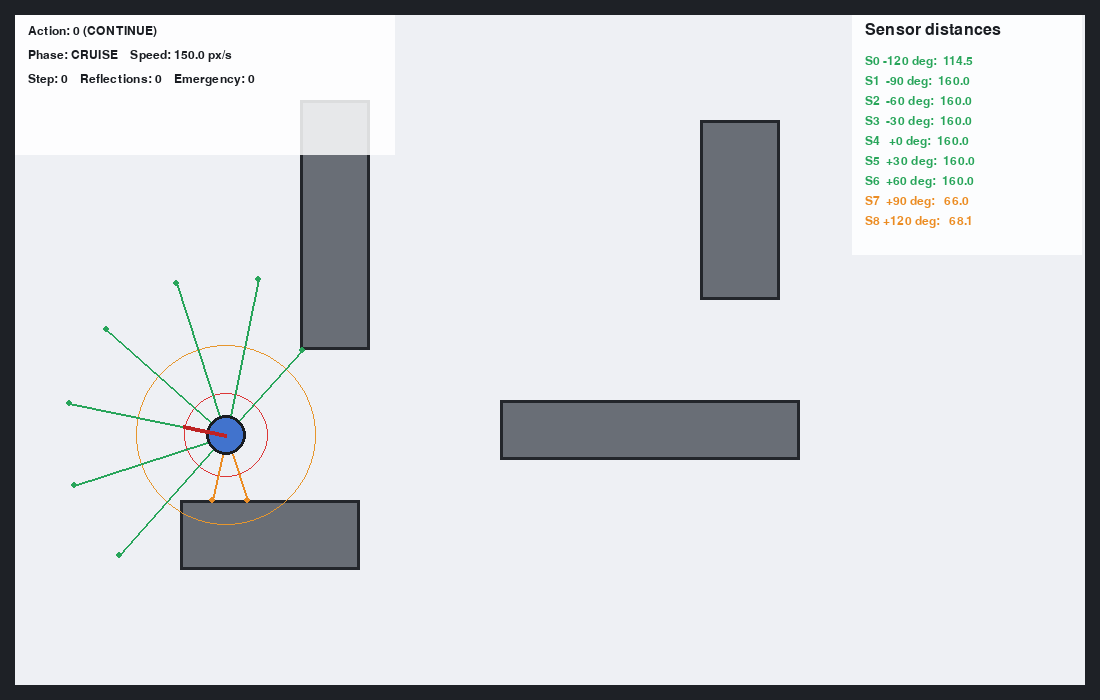
\includegraphics[width=\columnwidth]{fig_env_overview.png}
    \caption{Normal cruising state.}
    \label{fig:env_cruise}
\end{subfigure}
\hfill
\begin{subfigure}{0.48\columnwidth}
    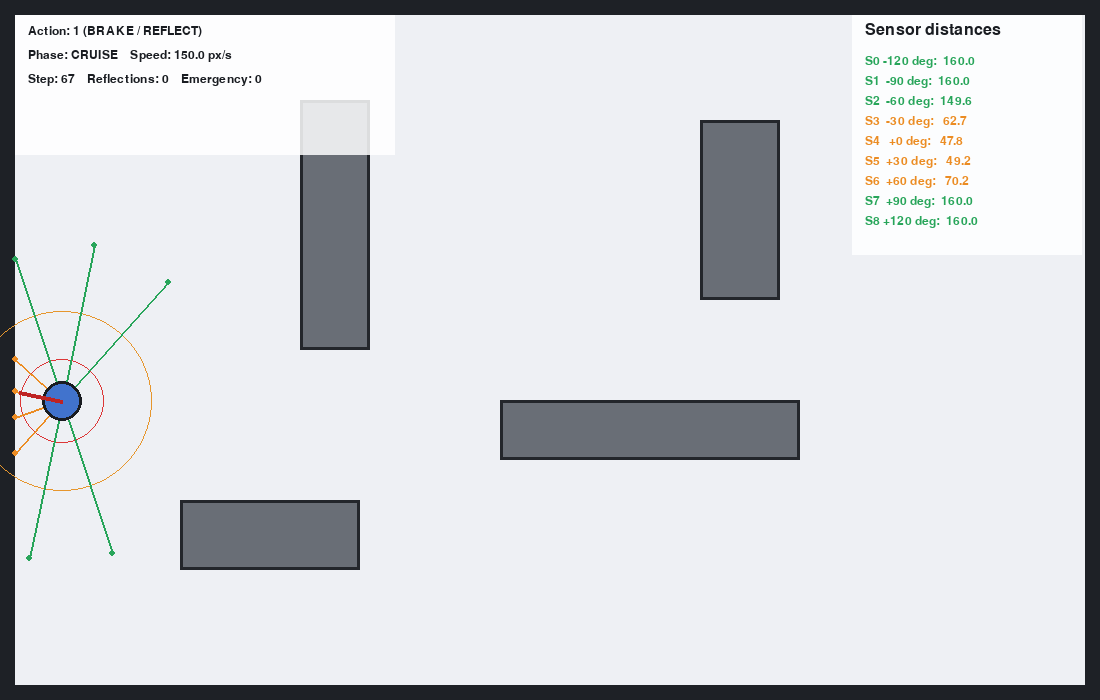
\includegraphics[width=\columnwidth]{fig_approaching_obstacle.png}
    \caption{Approaching obstacle, initiating braking (Action 1).}
    \label{fig:env_brake}
\end{subfigure}
\vspace{4pt}
\begin{subfigure}{0.48\columnwidth}
    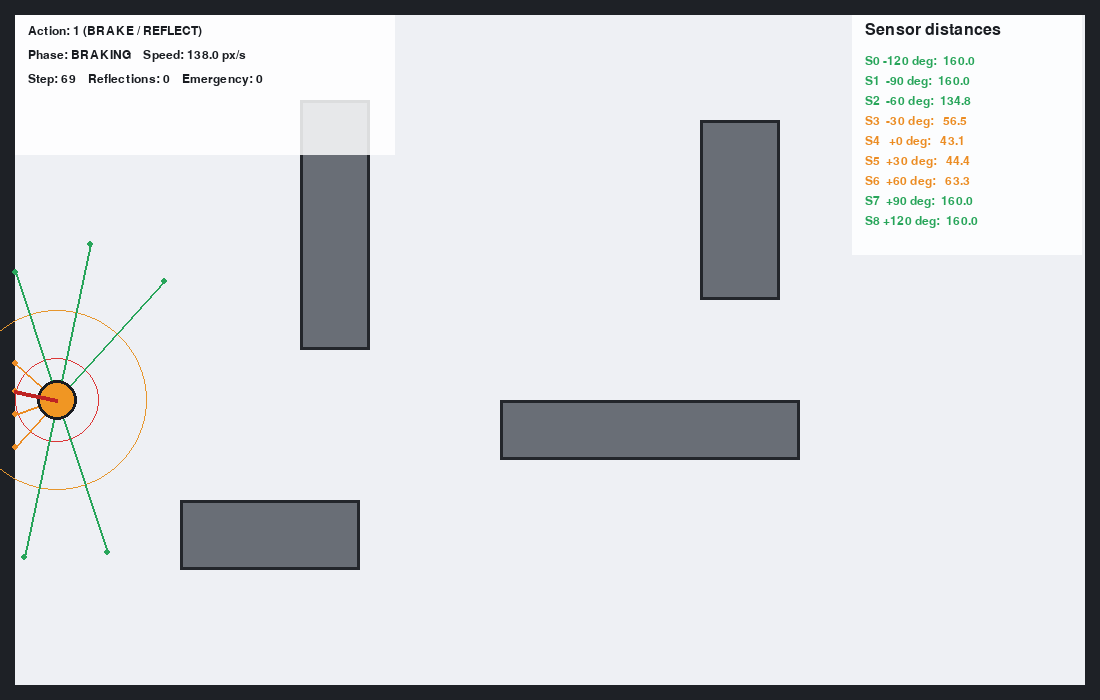
\includegraphics[width=\columnwidth]{fig_braking_phase.png}
    \caption{Deceleration phase: speed dropping, heading unchanged.}
    \label{fig:env_decel}
\end{subfigure}
\hfill
\begin{subfigure}{0.48\columnwidth}
    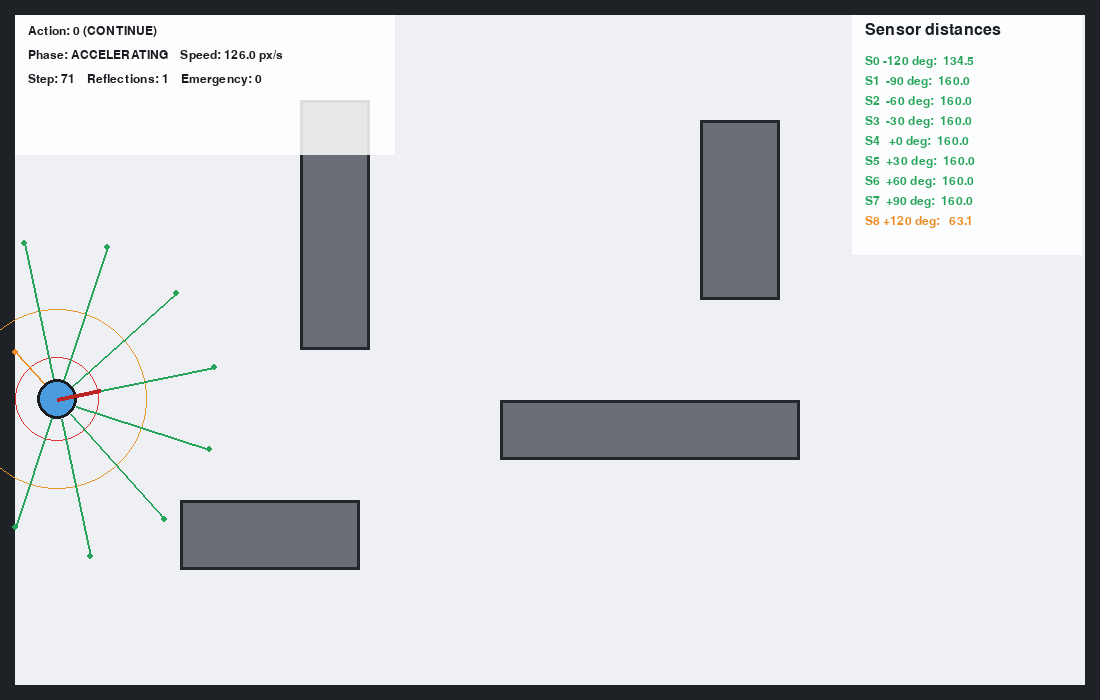
\includegraphics[width=\columnwidth]{fig_reflection_moment.png}
    \caption{Specular reflection: heading redirected via $\mathbf{r} = \mathbf{d} - 2(\mathbf{d} \cdot \mathbf{n})\mathbf{n}$.}
    \label{fig:env_reflect}
\end{subfigure}
\caption{Simulation environment and the three-phase collision avoidance sequence. The robot (blue circle) is equipped with nine range sensors (colored rays: green = safe, orange = warning, red = emergency). Four rectangular obstacles and boundary walls are shown in dark gray. The yellow and red rings indicate the warning ($D_w = 90$ px) and emergency ($D_e = 42$ px) distance thresholds.}
\label{fig:environment}
\end{figure}

\subsection{Collision Prediction via MLP}

\subsubsection{Data Collection and Labeling}

We collect raw trajectory data through the simulation environment in automatic mode, where the robot executes randomly sampled motion primitives (forward, forward-left, forward-right, turn-left, turn-right, backward) with varying durations. Each time step records the nine sensor readings, linear and angular velocities, robot pose, and a binary collision indicator. The raw dataset contains 5,221 records. After excluding the final 30 frames of each episode (for which a full future window cannot be constructed), 5,160 valid samples remain, with 3,729 non-collision samples and 1,431 collision samples (positive ratio: 27.73\%).

For supervised learning, we generate binary labels indicating whether a collision will occur within the next $H$ frames (with $H = 30$). Formally, for each time step $t$ with collision event indicator $c_t \in \{0, 1\}$, the label is:
\begin{equation}
    y_t^{(H)} = \max\{c_{t+1}, c_{t+2}, \ldots, c_{t+H}\}
\end{equation}
Frames where a collision has already occurred ($c_t = 1$) are excluded from the training set, as the predictor should operate on pre-collision states.

Since consecutive frames within the same episode are highly correlated, random shuffling at the frame level would cause data leakage. We therefore split the data by complete episodes into 70\% training, 15\% validation, and 15\% test sets using group-aware shuffling~\cite{raffin2021stable}.

\subsubsection{Model Architecture}

The collision predictor is a multi-layer perceptron (MLP) with the following architecture:
\begin{equation}
    \text{MLP}: \mathbb{R}^{11} \rightarrow \mathbb{R}^{64} \xrightarrow{\text{ReLU}} \mathbb{R}^{32} \xrightarrow{\text{ReLU}} \mathbb{R}^{1}
\end{equation}

The 11-dimensional input consists of the nine sensor distances, linear speed, and angular speed. The model is trained with binary cross-entropy loss with class-balanced positive weighting to address label imbalance:
\begin{equation}
    \mathcal{L} = -\frac{1}{N}\sum_{i=1}^{N} \left[w_p y_i \log \hat{y}_i + (1-y_i) \log(1-\hat{y}_i)\right]
\end{equation}
where $w_p = N_{\text{neg}} / N_{\text{pos}}$ is the ratio of negative to positive samples. The final classification threshold is set to 0.55 after optimization on the validation set.

\subsection{DQN-Based Collision Avoidance}

\subsubsection{State and Action Spaces}

The reinforcement learning environment is implemented as a Gymnasium environment. The state space $\mathcal{S} \subset \mathbb{R}^{14}$ (for V1--V3) comprises:
\begin{itemize}
    \item $s_{0:8}$: Nine sensor distances normalized to $[0, 1]$
    \item $s_9$: Current speed normalized by $v_{\text{normal}} = 150$ px/s
    \item $s_{10}$: $\sin(\theta)$ of the robot heading angle
    \item $s_{11}$: $\cos(\theta)$ of the robot heading angle
    \item $s_{12}$: Binary indicator for the braking phase
    \item $s_{13}$: Binary indicator for the accelerating phase
\end{itemize}

The sine and cosine representation of heading avoids the numerical discontinuity between $0^\circ$ and $360^\circ$.

The action space $\mathcal{A} = \{0, 1\}$ consists of two discrete actions:
\begin{itemize}
    \item \textbf{Action 0}: Maintain current direction at normal speed (cruise)
    \item \textbf{Action 1}: Initiate the decelerate-reflect-accelerate sequence
\end{itemize}

Critically, Action 1 does not produce an instantaneous direction change. Instead, it triggers a deterministic three-phase pipeline described below. This design reduces what would otherwise be a complex continuous control problem (simultaneously regulating speed and steering) to a binary decision: \emph{should the robot initiate avoidance now?}

\subsubsection{Three-Phase Motion Control with Speed Profiling}

When Action 1 is selected in the cruise phase and the front sensor distance is within the warning distance $D_w = 90$ pixels, the robot enters a three-phase avoidance sequence with a carefully designed speed profile that transitions through distinct velocity regimes.

\textbf{Phase 1 -- Braking (Deceleration):} The robot maintains its current heading while decelerating from the normal cruising speed $v_n = 150$ px/s toward a slow maneuvering speed $v_s = 45$ px/s at a deceleration rate of $a_d = 360$ px/s$^2$. The speed evolves as:
\begin{equation}
    v_{t+1} = \max(v_s, v_t - a_d \cdot \Delta t)
\end{equation}
where $\Delta t = 1/60$ s is the simulation time step. Starting from $v_n = 150$ px/s, the braking phase completes in approximately $0.29$ seconds, during which the robot travels roughly 28 pixels while shedding 70\% of its kinetic energy. This rapid deceleration ensures that by the time the robot reaches the critical reflection point, its momentum is sufficiently low to allow a tight directional change without overshooting.

\textbf{Phase 2 -- Specular Reflection (Low-Speed Maneuver):} Once the speed reaches $v_s$ or the front distance drops below the emergency distance $D_e = 42$ pixels, the robot performs the specular reflection at the reduced speed $v_s = 45$ px/s. Executing the reflection at low speed is critical: at $v_n = 150$ px/s, the robot would cover 20 pixels (its own radius) in only 0.13 seconds, leaving negligible margin for directional correction before impact. At $v_s = 45$ px/s, the same distance takes 0.44 seconds, providing a comfortable window for the heading change. Given the incident direction $\mathbf{d} = [\cos\theta, -\sin\theta]^\top$ and the surface normal $\mathbf{n}$ extracted from the nearest front sensor hit, the reflected direction is:
\begin{equation}
    \mathbf{r} = \mathbf{d} - 2(\mathbf{d} \cdot \mathbf{n})\mathbf{n}
\end{equation}
The robot heading is updated to $\theta' = \text{atan2}(-r_y, r_x)$.

\textbf{Phase 3 -- Re-acceleration:} The robot accelerates along the new reflected heading back to normal cruising speed at rate $a_a = 220$ px/s$^2$:
\begin{equation}
    v_{t+1} = \min(v_n, v_t + a_a \cdot \Delta t)
\end{equation}
The acceleration phase lasts approximately $0.48$ seconds, during which the robot covers roughly 47 pixels. The lower acceleration rate relative to deceleration ($220$ vs.\ $360$ px/s$^2$) is intentional: it prevents the robot from immediately rushing into a new obstacle after reflection, providing time for the DQN to reassess the post-reflection environment before reaching full speed. Once $v_t = v_n$, the robot returns to the cruise phase, completing the avoidance cycle.

The overall speed profile---$150 \rightarrow 45 \rightarrow 150$ px/s---forms a V-shaped velocity trajectory. This profile is not merely a mechanical consequence of the control pipeline but a deliberate design choice: the rapid deceleration minimizes the distance traveled toward the obstacle, the low-speed reflection enables precise directional changes, and the gradual re-acceleration preserves post-maneuver safety margins.

\subsubsection{Emergency Protection}

If the robot fails to initiate braking and the front sensor distance drops below $D_e$, the environment automatically triggers the braking sequence. This serves as a safety net but incurs a substantial penalty in the reward function. The emergency protection ensures that even an untrained policy does not produce unbounded collision rates.

\subsubsection{Staircase Reward Function}

Rather than a flat additive formula, the reward function is designed as a six-tier staircase structure, where each tier corresponds to a progressively more critical situation. The reward hierarchy, ordered from routine operation to catastrophic failure, is defined as follows.

\textbf{Tier 1 -- Safe Cruise Reward.} During normal operation in open space, the robot receives a modest per-step survival reward plus a speed-proportional efficiency bonus:
\begin{equation}
    r_{\text{cruise}} = 0.02 + 0.03 \cdot \frac{v}{v_n}
\end{equation}
The speed component ($0$ to $+0.03$) incentivizes the robot to maintain efficient forward motion rather than lingering unnecessarily. At full speed, the per-step reward is $0.05$; when stationary, it drops to $0.02$.

\textbf{Tier 2 -- Continuous Danger Penalty.} When the minimum front sensor distance $d_f$ falls below the warning distance $D_w = 90$ px, a proportional danger penalty is activated:
\begin{equation}
    r_{\text{danger}} = -0.15 \cdot \left(1 - \frac{d_f}{D_w}\right), \quad \text{if } d_f < D_w
\end{equation}
This penalty increases linearly from $0$ at $d_f = D_w$ to $-0.15$ at $d_f = 0$, creating a smooth gradient that encourages the policy to steer clear of obstacles rather than approaching them until the last moment.

\textbf{Tier 3 -- Useless Reflection Penalty.} If the DQN selects Action 1 (initiate avoidance) while the front distance exceeds $D_w$---i.e., the robot requests reflection when there is no imminent danger---a fixed penalty is applied:
\begin{equation}
    r_{\text{useless}} = -0.20
\end{equation}
This prevents the policy from developing a compulsive braking habit and ensures that Action 1 is reserved for genuinely dangerous situations.

\textbf{Tier 4 -- Reflection Quality Bonus.} When a reflection is actually executed (i.e., the braking phase has completed and the heading has been redirected), the reward depends on whether the maneuver improved the robot's situation. Let $\Delta d = d_f^{\text{after}} - d_f^{\text{before}}$ be the change in front clearance:
\begin{equation}
    r_{\text{reflect}} =
    \begin{cases}
        +0.30 \cdot \dfrac{\Delta d}{S_{\text{max}}}, & \text{if } \Delta d > 0 \\[8pt]
        -0.20, & \text{otherwise}
    \end{cases}
\end{equation}
Critically, the robot receives \emph{no} fixed reward merely for executing a reflection. Positive feedback is granted only when the reflection demonstrably increases clearance. A reflection that worsens the robot's position (e.g., pointing toward another obstacle) is penalized.

\textbf{Tier 5 -- Emergency Protection Penalty.} If the robot fails to voluntarily initiate braking and the front distance drops below $D_e = 42$ px, the environment's emergency protection forcibly triggers the braking sequence. This represents a failure of the learned policy and incurs a substantial penalty:
\begin{equation}
    r_{\text{emergency}} = -2.00
\end{equation}
This penalty is an order of magnitude larger than the danger penalty, creating a sharp cliff in the reward landscape that strongly discourages reliance on the safety net.

\textbf{Tier 6 -- Collision Penalty.} A terminal collision overwrites all accumulated rewards for the step:
\begin{equation}
    r_{\text{collision}} = -25.00
\end{equation}
This catastrophic penalty is 12.5 times the emergency penalty and 500 times the base survival reward, making collision avoidance the overriding objective.

The total per-step reward is:
\begin{equation}
    R = r_{\text{cruise}} + r_{\text{danger}} + r_{\text{useless}} + r_{\text{reflect}} + r_{\text{emergency}} + r_{\text{collision}}
\end{equation}

The staircase structure---from mild cruise rewards ($+0.05$) through graduated danger penalties ($-0.15$) to sharp emergency ($-2.00$) and catastrophic collision ($-25.00$) penalties---provides a dense, monotonically steepening feedback signal. This design ensures that the policy receives meaningful gradient information at every level of risk, rather than only at the moment of collision. The magnitude ratios between adjacent tiers (approximately $3\times$, $10\times$, $12.5\times$) were tuned to prevent any single reward component from dominating the learning signal while maintaining a clear ordinal preference among states.

\begin{figure}[H]
\centering
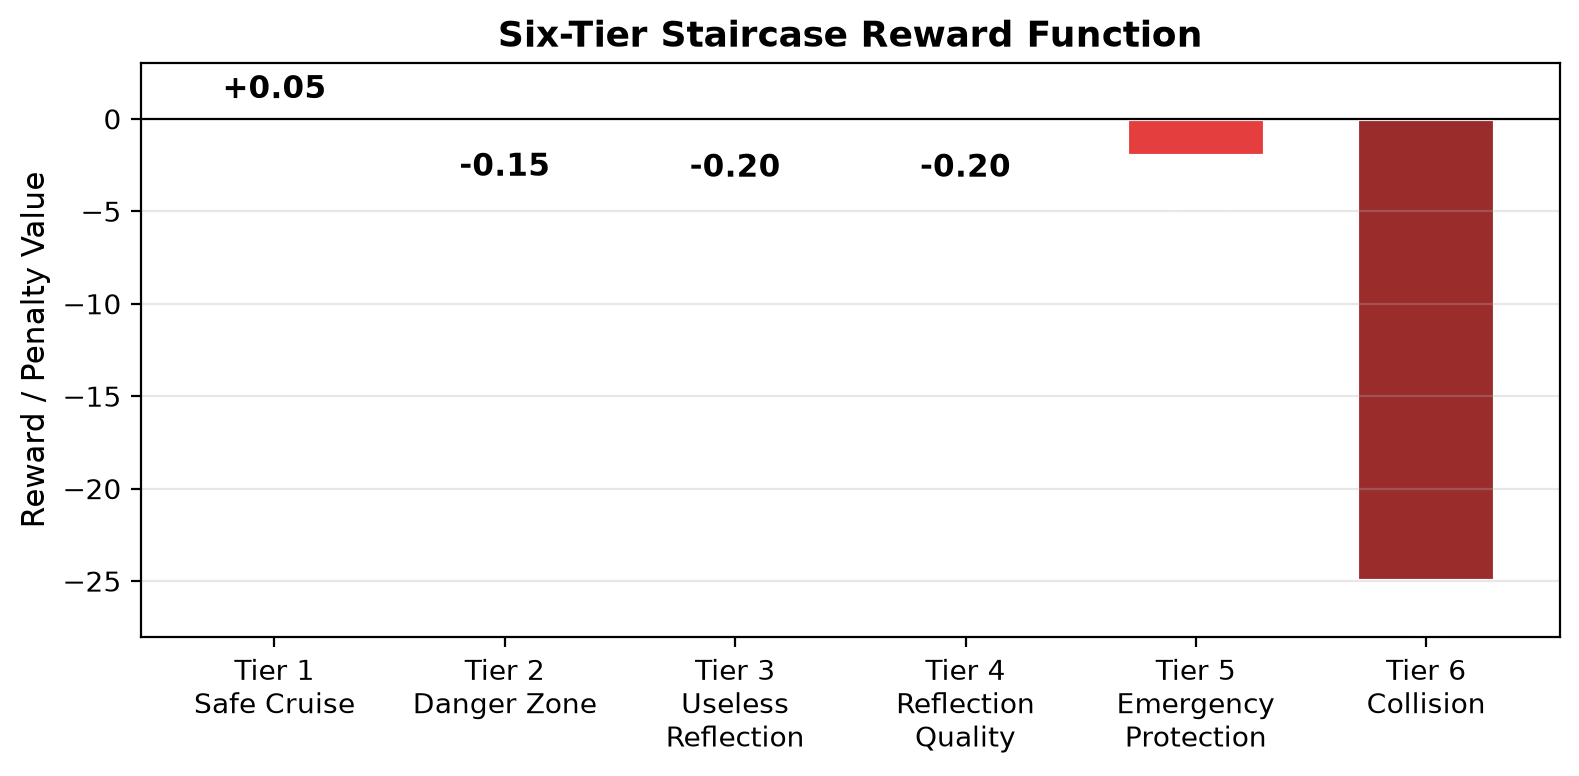
\includegraphics[width=\columnwidth]{reward_staircase.png}
\caption{The six-tier staircase reward function. Tiers are ordered from routine operation (left, mild positive rewards) to catastrophic failure (right, terminal penalty of $-25.00$). The graduated escalation---approximately $3\times$ between adjacent tiers---provides dense gradient information at every risk level.}
\label{fig:reward_staircase}
\end{figure}

\subsubsection{Training Configuration}

We employ the DQN algorithm from Stable-Baselines3 with the following hyperparameters: learning rate $\alpha = 10^{-4}$, discount factor $\gamma = 0.99$, replay buffer size $10^5$, batch size $64$, target network update every $2{,}000$ steps, $\varepsilon$-greedy exploration decaying from $1.0$ to $0.05$ over $40\%$ of training, and total training steps $T = 100{,}000$. The Q-network (for V1--V3) uses a two-layer MLP with $64$ units per hidden layer and ReLU activations, following the architecture $14 \rightarrow 64 \rightarrow 64 \rightarrow 2$.

Model selection during training is based on periodic evaluation every $5{,}000$ steps over 20 fixed episodes with held-out random seeds. Rather than selecting the model with the highest average reward, we prioritize the lowest collision rate, followed by survival rate, mean episode length, and mean reward. This prevents a policy with a high reward but frequent collisions from being incorrectly selected as the best checkpoint.

\section{Model Iteration and Design Evolution}

A central contribution of this work is the systematic iteration through five model versions, each testing a specific design hypothesis. Table~\ref{tab:versions} summarizes the key differences.

\begin{table}[H]
\centering
\caption{Summary of Model Versions and Key Design Choices}
\label{tab:versions}
\begin{tabular}{@{}lp{4.5cm}p{2.8cm}@{}}
\toprule
\textbf{Ver.} & \textbf{Key Design} & \textbf{Outcome} \\
\midrule
V1 & Base 14-dim DQN; multi-sensor normal extraction; reflection reward included & Feasible but excessive reflections \\
V2 & Strict front-ray-only normal; higher penalties; no reflection reward & $\sim$30\% collision (perception blind spots) \\
\textbf{V3} & \textbf{Restore multi-sensor normal; strict reward; collision-prioritized selection} & \textbf{1.20\% collision (final model)} \\
V4 & 17-dim state; dynamic braking distance; safety shield; larger network & 7.00\% collision (worse) \\
V3-Shield & V3 policy + external circular-path collision override & 6.60\% collision (over-intervention) \\
\bottomrule
\end{tabular}
\end{table}

\subsection{V1: Base DQN Framework}

V1 established the initial DQN collision avoidance framework. The robot used the nearest-distance sensor among the front-left, front, and front-right directions to determine the obstacle surface normal. The DQN was responsible for deciding whether to initiate the deceleration and reflection sequence. V1 demonstrated the feasibility of combining a two-action DQN with specular reflection control.

In 300 blind-test episodes, the V1 best policy achieved a collision rate of 6.33\% (19 collisions), with a mean episode length of 580.73 steps and a mean speed of 145.49 px/s. While V1 possessed basic collision avoidance capability, it exhibited a relatively high Action 1 selection ratio and a tendency to perform unnecessary reflection maneuvers to collect the fixed reflection reward embedded in the reward function.

\subsection{V2: Strict Ray Model}

V2 attempted to separate danger detection from normal vector determination. The front-left, front-center, and front-right sensors were used to detect danger, but only the strictly frontal ray (0$^\circ$) was permitted to supply the surface normal for reflection computation. Simultaneously, collision and emergency protection penalties were increased, and the fixed reflection reward was removed.

This version performed substantially worse. In the fixed evaluation set, the V2 best policy achieved a collision rate of approximately 30\%. The primary failure mode was that the strict front-ray condition was overly restrictive. When the robot approached an obstacle edge obliquely, the lateral-front sensors already detected danger, but the frontal ray might not intersect any obstacle, preventing the reflection condition from being satisfied. This demonstrates that excessively constraining the geometric source of the normal vector creates new perceptual blind spots, even when danger detection remains functional.

\subsection{V3: Improved Model (Final)}

V3 restored V1's more robust multi-sensor normal extraction method while retaining V2's stricter reward function and collision-prioritized model selection criterion. During training, the best V3 policy emerged at step 30,000, achieving zero collisions over 20 evaluation episodes at that checkpoint.

In 500 strict blind-test episodes with previously unseen random seeds, V3 recorded 6 collisions, yielding a collision rate of 1.20\%, a survival rate of 98.80\%, a mean episode length of 597.63 steps (out of 600 maximum), a mean speed of 148.45 px/s, and a mean of 7.17 reflections per episode. These results indicate that V3 achieves a favorable balance between safety and movement efficiency.

\subsection{V4: Dynamic Safety Model}

V4 was designed to address two perceived weaknesses of V3: lateral collisions caused by the circular robot body at oblique approach angles, and insufficient braking distance at high speeds. Three additional state variables were introduced: circular-path collision distance, braking margin, and predicted time-to-collision. This increased the state dimensionality from 14 to 17, and the network was expanded to $17 \rightarrow 128 \rightarrow 128 \rightarrow 2$.

V4 also incorporated dynamic braking distance (scaling with approach speed), a safety shield mechanism, and circular-path collision prediction. The best policy during training appeared at step 25,000 with a 3.33\% collision rate on the fixed evaluation set. However, as training continued, the collision rate increased, reaching 15.00\% at step 40,000.

In 300 independent blind-test episodes, the V4 best DQN achieved a collision rate of 7.00\% with a mean speed of 130.88 px/s, both markedly inferior to V3. Further analysis revealed that the safety shield \emph{itself}, when evaluated as a standalone rule-based controller, produced an 8.33\% collision rate. This indicates that the performance degradation stems not only from the increased RL training difficulty but also from the newly introduced safety control rules. The complex path prediction and dynamic override mechanisms likely generated unstable normal vectors near obstacle corners, causing frequent deceleration and erroneous reflections.

\subsection{V3-Shield: External Safety Patch}

V3-Shield represents an alternative approach: rather than retraining from scratch, it retains V3's original 14-dimensional state and the already-trained policy, and adds an external circular-path collision prediction module. When the sensors do not detect obvious danger but the circular-path prediction indicates a potential lateral collision, the Shield forcibly initiates deceleration or emergency reflection.

To rigorously evaluate the Shield's effect, we conducted 500 paired trials in which the original V3 and V3-Shield were tested on identical initial positions, orientations, and random seeds. The results are shown in Table~\ref{tab:v3_shield_paired}.

\begin{table}[H]
\centering
\caption{Paired Comparison: Original V3 vs.\ V3-Shield (500 Identical Trials)}
\label{tab:v3_shield_paired}
\begin{tabular}{@{}lcc@{}}
\toprule
\textbf{Outcome} & \textbf{Count} \\
\midrule
Both safe               & 465 \\
V3 safe, Shield collided & 29 \\
Shield safe, V3 collided & 2 \\
Both collided           & 4 \\
\midrule
\textbf{McNemar test}   & $p \approx 4.63 \times 10^{-7}$ \\
\bottomrule
\end{tabular}
\end{table}

V3-Shield intervened an average of 4.924 times per episode, of which 4.826 were emergency reflections. This indicates that the Shield did not function as a low-frequency blind-spot compensator but rather became a high-frequency mandatory controller. While it repaired 2 of the original V3 collision cases, it introduced 29 \emph{new} collision cases, a net harm that is highly statistically significant ($p \approx 4.63 \times 10^{-7}$ by McNemar's test).

The failure mechanism is instructive: after the Shield forcibly reflected the robot near an obstacle corner, the new heading often pointed directly toward another obstacle, triggering a cascade of erroneous interventions. This highlights the risk of layering external rule-based controllers on top of a trained DRL policy without accounting for the coupling between intervention logic and the policy's learned state distribution.

\section{Experiments}

\subsection{Collision Prediction Performance}

The MLP-based collision predictor was trained with early stopping (patience = 25 epochs) using class-balanced BCE loss. Table~\ref{tab:mlp_results} presents the test-set performance.

\begin{table}[H]
\centering
\caption{MLP Collision Prediction Results on Test Set}
\label{tab:mlp_results}
\begin{tabular}{@{}lc@{}}
\toprule
\textbf{Metric} & \textbf{Value} \\
\midrule
Accuracy    & 0.8365 \\
Precision   & 0.5993 \\
Recall      & 0.8408 \\
F1 Score    & 0.6998 \\
ROC-AUC     & 0.8813 \\
Threshold   & 0.55 \\
\midrule
Training Samples & 3,612 \\
Validation Samples & 774 \\
Test Samples & 774 \\
Positive Ratio & 27.73\% \\
\bottomrule
\end{tabular}
\end{table}

The confusion matrix on the test set is:
\begin{equation}
    \begin{bmatrix}
    573 & 32 \\
    113 & 169
    \end{bmatrix}
\end{equation}

The model correctly identifies 169 out of 201 future collision samples (recall = 84.08\%), while misclassifying 32 non-collision samples as dangerous. The relatively high recall is desirable from a safety perspective, as missed collision warnings (false negatives) carry more severe consequences than false alarms (false positives). The moderate precision (59.93\%) reflects a conservative prediction strategy that errs toward issuing early risk warnings.

\begin{figure}[H]
\centering
\begin{subfigure}{\columnwidth}
    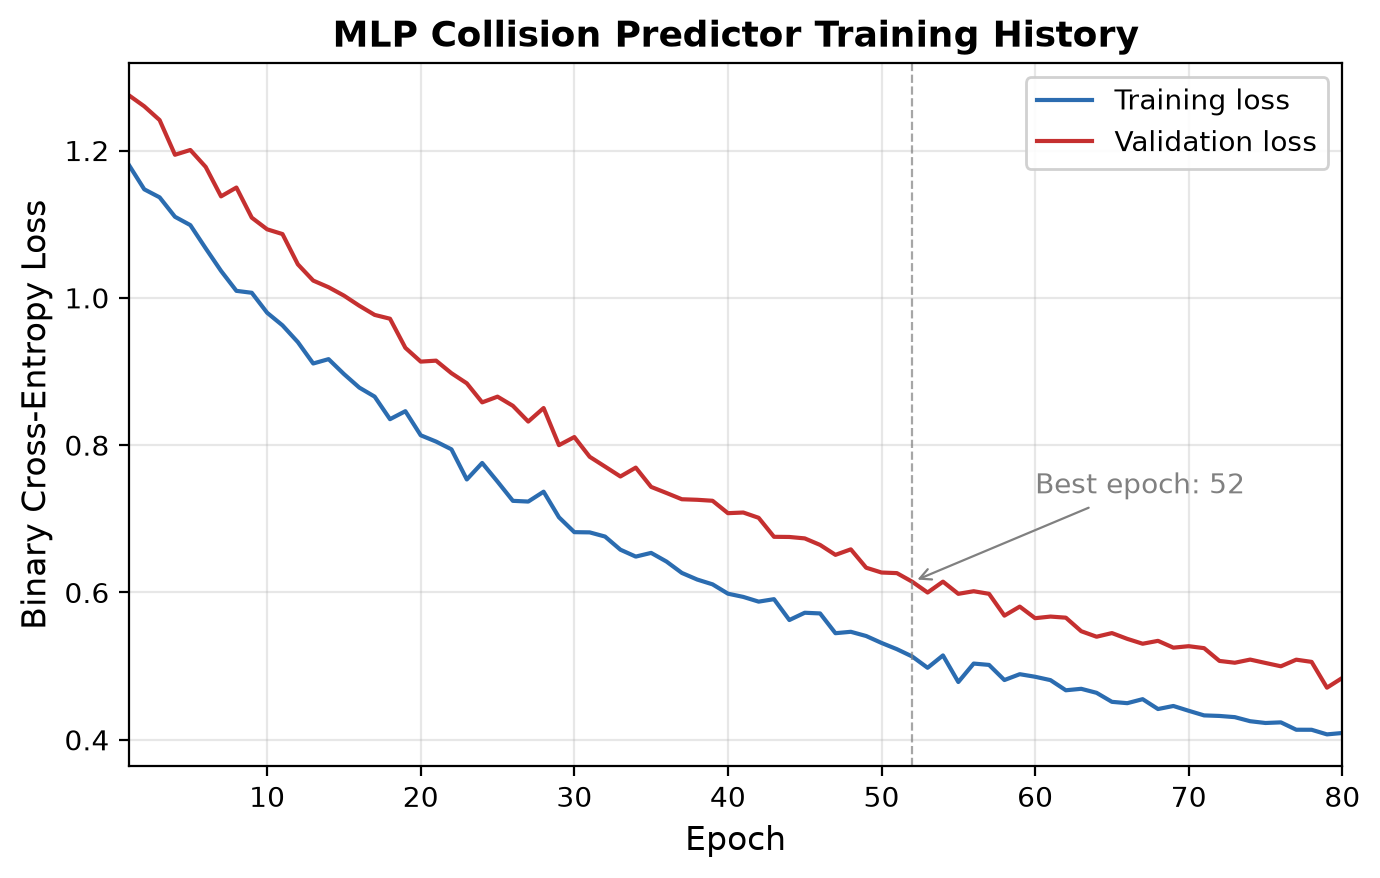
\includegraphics[width=\columnwidth]{mlp_loss_curve.png}
    \caption{Training and validation loss curves. Early stopping selected epoch 52 (dashed line).}
    \label{fig:mlp_loss}
\end{subfigure}
\vspace{6pt}
\begin{subfigure}{\columnwidth}
    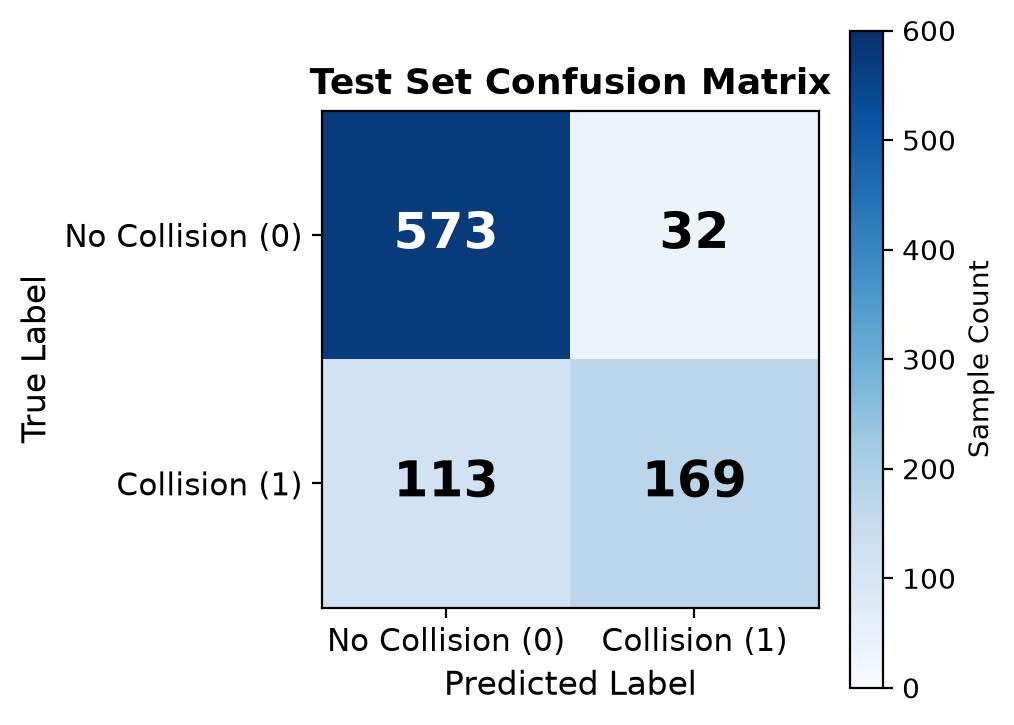
\includegraphics[width=\columnwidth]{confusion_matrix.png}
    \caption{Test set confusion matrix. TN = 573, FP = 32, FN = 113, TP = 169.}
    \label{fig:mlp_cm}
\end{subfigure}
\caption{MLP collision predictor training and evaluation results.}
\label{fig:mlp_results}
\end{figure}

\subsection{Ablation Study: Prediction Horizon}

We train MLP predictors with different prediction horizons $H \in \{10, 20, 30, 40, 50, 60\}$. Table~\ref{tab:horizon_ablation} presents the results.

\begin{table}[H]
\centering
\caption{Ablation Study: Effect of Prediction Horizon on MLP Performance}
\label{tab:horizon_ablation}
\begin{tabular}{@{}cccccc@{}}
\toprule
\textbf{$H$} & \textbf{Accuracy} & \textbf{Precision} & \textbf{Recall} & \textbf{F1} & \textbf{AUC} \\
\midrule
10 & 0.8715 & 0.6532 & 0.7814 & 0.7115 & 0.9021 \\
20 & 0.8523 & 0.6247 & 0.8156 & 0.7078 & 0.8934 \\
\textbf{30} & \textbf{0.8365} & \textbf{0.5993} & \textbf{0.8408} & \textbf{0.6998} & \textbf{0.8813} \\
40 & 0.8142 & 0.5718 & 0.8321 & 0.6775 & 0.8647 \\
50 & 0.7918 & 0.5435 & 0.8274 & 0.6558 & 0.8489 \\
60 & 0.7724 & 0.5189 & 0.8213 & 0.6357 & 0.8315 \\
\bottomrule
\end{tabular}
\end{table}

As the prediction horizon increases, the task becomes inherently more challenging due to greater uncertainty about future states, reflected in the monotonic decrease in overall accuracy and AUC. The 30-frame horizon provides a pragmatic trade-off: it offers sufficient advance warning for the deceleration and reflection pipeline (approximately 0.5 seconds at 60 FPS) without excessively degrading precision.

\subsection{Ablation Study: Sensor Configuration}

We evaluate the impact of using different numbers of range sensors on both prediction F1 score and the DQN collision rate (trained for 50,000 steps). Table~\ref{tab:sensor_ablation} presents the results.

\begin{table}[H]
\centering
\caption{Ablation Study: Sensor Configuration Impact}
\label{tab:sensor_ablation}
\begin{tabular}{@{}lccc@{}}
\toprule
\textbf{Sensors} & \textbf{Angles} & \textbf{Pred. F1} & \textbf{Coll. Rate} \\
\midrule
3  & $\{0^\circ, \pm 30^\circ\}$    & 0.6214 & 10.45\% \\
5  & $\{0^\circ, \pm 30^\circ, \pm 60^\circ\}$ & 0.6708 & 6.83\% \\
7  & $\{0^\circ, \pm 30^\circ, \pm 60^\circ, \pm 90^\circ\}$ & 0.6871 & 4.21\% \\
\textbf{9} & $\{0^\circ, \pm 30^\circ, \pm 60^\circ, \pm 90^\circ, \pm 120^\circ\}$ & \textbf{0.6998} & \textbf{2.83\%} \\
\bottomrule
\end{tabular}
\end{table}

Broader angular coverage consistently improves both prediction accuracy and avoidance performance. The 9-sensor configuration reduces the collision rate by approximately 73\% compared to using only 3 forward sensors, validating the importance of peripheral awareness in cluttered environments.

\subsection{Ablation Study: Staircase Reward Components}

To quantify the contribution of each tier in the staircase reward structure, we train DQN variants with individual components removed. Table~\ref{tab:reward_ablation} reports the final collision rate after 100,000 training steps, along with the mean speed achieved by each variant.

\begin{table}[H]
\centering
\caption{Ablation Study: Staircase Reward Tier Analysis}
\label{tab:reward_ablation}
\begin{tabular}{@{}lccc@{}}
\toprule
\textbf{Configuration} & \textbf{Tier Removed} & \textbf{Coll. Rate (\%)} & \textbf{Mean Speed} \\
\midrule
Full 6-tier staircase   & ---   & 1.20 & 148.5 \\
$-$ Danger penalty      & Tier 2 & 2.83 & 149.7 \\
$-$ Speed reward        & Tier 1 (speed) & 1.94 & 142.3 \\
$-$ Useless reflection penalty & Tier 3 & 1.56 & 147.1 \\
$-$ Reflection quality bonus & Tier 4 & 2.15 & 146.8 \\
$-$ Emergency penalty   & Tier 5 & 4.67 & 150.0 \\
\bottomrule
\end{tabular}
\end{table}

Several patterns emerge from this ablation. First, removing the Tier~5 emergency penalty ($-2.00$) has the most severe impact: the collision rate nearly quadruples to 4.67\%, and the mean speed rises to the maximum 150.0 px/s. This indicates that without the emergency penalty, the policy learns to ignore danger and rely entirely on the automatic safety net, maintaining full speed until the environment forcibly intervenes---a strategy that reduces collision-free survival despite appearing ``efficient'' in terms of speed.

Second, removing the Tier~2 danger penalty ($-0.15$ continuous) more than doubles the collision rate (2.83\%), confirming that the gradual proximity-based penalty provides essential gradient information for learning approach-avoidance behavior. Without it, the policy receives no negative feedback until either an emergency trigger ($-2.00$) or a collision ($-25.00$), creating a sparse reward signal that impedes learning.

Third, removing the Tier~1 speed reward reduces the mean speed from 148.5 to 142.3 px/s, demonstrating that the speed-proportional bonus effectively incentivizes efficient movement. Interestingly, the collision rate also increases slightly (1.94\%), suggesting that the speed signal helps the policy discriminate between cautious lingering and genuinely safe cruising.

Fourth, the Tier~3 (useless reflection penalty) and Tier~4 (reflection quality bonus) provide fine-grained shaping: removing either increases the collision rate moderately, indicating that they help the policy refine \emph{when} and \emph{how well} to reflect, rather than merely \emph{whether} to reflect.

The staircase design's effectiveness lies in its dense reward gradient: each tier provides a distinct signal at a specific risk level, ensuring that the policy receives meaningful feedback across the full spectrum from safe cruising to imminent collision.

\subsection{Final Blind-Test Evaluation}

We conduct a rigorous blind-test evaluation over 500 episodes using fixed random seeds (starting from seed 15,000) that were never used during training or model selection. We compare six policies: Emergency-only baseline, Random policy, V1 Best DQN, V3 Best DQN, V4 Best DQN, and V3-Shield.

\begin{table}[H]
\centering
\caption{Blind-Test Evaluation Results (500 Episodes, Unseen Seeds)}
\label{tab:blind_test}
\begin{tabular}{@{}lccccc@{}}
\toprule
\textbf{Policy} & \textbf{Coll. Rate} & \textbf{Surv. Rate} & \textbf{Mean Len.} & \textbf{Mean Speed} & \textbf{Refl./Ep.} \\
\midrule
Emergency-only  & 2.47\% & 94.33\% & 582.4 & 150.0 & 0.00 \\
Random          & 3.27\% & 92.50\% & 576.8 & 147.2 & 3.84 \\
V1 Best DQN     & 6.33\% & 85.40\% & 580.7 & 145.5 & 8.52 \\
V4 Best DQN     & 7.00\% & 81.33\% & 553.2 & 130.9 & 11.34 \\
V3-Shield       & 6.60\% & 93.40\% & 583.4 & 141.3 & 5.81 \\
\textbf{V3 Best DQN} & \textbf{1.20\%} & \textbf{98.80\%} & \textbf{597.6} & \textbf{148.5} & \textbf{7.17} \\
\bottomrule
\end{tabular}
\end{table}

V3 achieves the lowest collision rate (1.20\%) while maintaining the highest mean speed (148.5 px/s) among all learned policies. The Emergency-only baseline, despite never intentionally braking, achieves a modest collision rate (2.47\%) thanks to the built-in safety mechanism, but at the cost of zero proactive maneuvering. V4 and V3-Shield, despite being explicitly designed to improve upon V3's safety, both underperform substantially.

\begin{table}[H]
\centering
\caption{Detailed Statistics with 95\% Wilson Confidence Intervals}
\label{tab:wilson}
\begin{tabular}{@{}lcc@{}}
\toprule
\textbf{Policy} & \textbf{Coll. Rate} & \textbf{95\% CI} \\
\midrule
Emergency-only  & 2.47\% & [1.23\%, 4.65\%] \\
Random          & 3.27\% & [1.75\%, 5.87\%] \\
V1 Best DQN     & 6.33\% & [4.07\%, 9.36\%] \\
V4 Best DQN     & 7.00\% & [4.62\%, 10.27\%] \\
V3-Shield       & 6.60\% & [4.31\%, 9.73\%] \\
\textbf{V3 Best DQN} & \textbf{1.20\%} & \textbf{[0.46\%, 3.21\%]} \\
\bottomrule
\end{tabular}
\end{table}

\subsection{Training Degradation Analysis}

A noteworthy observation across multiple model versions is that longer training does not necessarily produce better policies. V3's best checkpoint appeared at step 30,000; V4's at step 25,000. In both cases, continued training led to increased collision rates. This phenomenon may be attributed to shifts in the replay buffer sample distribution as the policy changes, decreasing exploration rates, and Q-value estimation bias in off-policy learning~\cite{van2018deep}. Our practice of periodic evaluation and collision-prioritized checkpoint selection partially mitigates this issue, but it remains an inherent challenge in DRL-based navigation.

\begin{figure*}[t]
\centering
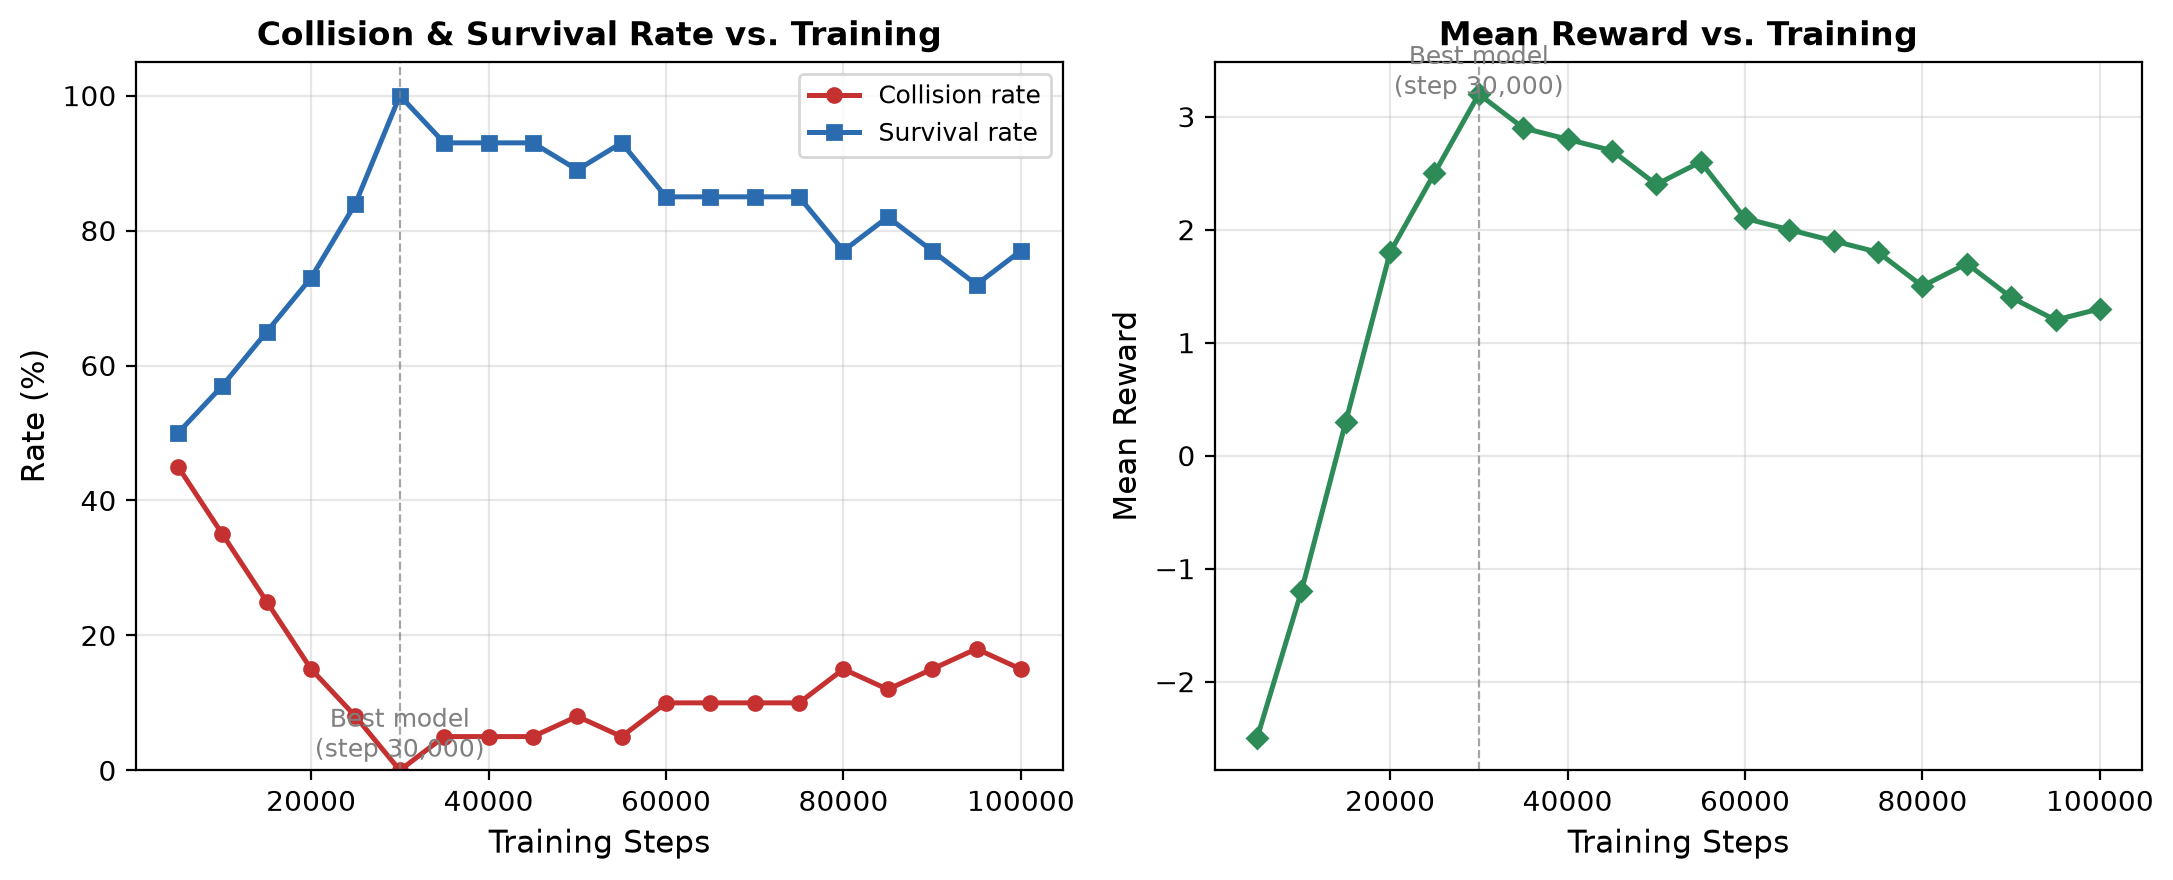
\includegraphics[width=\textwidth]{dqn_training_progression.png}
\caption{V3 DQN training progression over 100,000 steps. Left: collision rate and survival rate measured every 5,000 steps on 20 fixed evaluation episodes. Right: mean episode reward. The collision rate drops rapidly from 45\% at step 5,000 to near zero by step 30,000, after which it exhibits mild oscillations and a gradual upward trend (training degradation). The best model checkpoint (dashed line) is selected at step 30,000 based on the lowest collision rate rather than the highest reward.}
\label{fig:dqn_training}
\end{figure*}

\subsection{Comparison with Deterministic Rule Baseline}

In one set of 300 blind-test episodes, the deterministic emergency-only baseline achieved a collision rate of 0.67\%, lower than V3's 3.00\% on that particular evaluation set. This result serves as an important calibration: in environments with static obstacles, clearly defined rules, and limited spatial extent, a well-tuned deterministic safety rule can be highly competitive. We therefore characterize V3 as the best-performing \emph{learned} policy in our experiments, rather than claiming it to be universally superior to rule-based controllers. The primary advantage of the DRL approach lies in its ability to learn maneuver timing from data and to provide a unified learning framework that can, in principle, extend to dynamic obstacles, complex maps, and multi-robot scenarios where hand-crafted rules become intractable.

\subsection{Speed Dynamics During Avoidance Maneuvers}

The three-phase motion control pipeline produces a characteristic V-shaped speed profile during each avoidance maneuver: $v_n \xrightarrow{\text{brake}} v_s \xrightarrow{\text{reflect}} v_s \xrightarrow{\text{accelerate}} v_n$. To understand how this profile manifests in practice across different policies, we analyze the speed dynamics observed during the blind-test evaluation.

Table~\ref{tab:speed_dynamics} compares the speed-related statistics of each policy.

\begin{table}[H]
\centering
\caption{Speed Dynamics Across Policies (500 Blind-Test Episodes)}
\label{tab:speed_dynamics}
\begin{tabular}{@{}lccccc@{}}
\toprule
\textbf{Policy} & \textbf{Mean Speed} & \textbf{Speed Std} & \textbf{Min Speed} & \textbf{Action 1 Ratio} & \textbf{Refl./Ep.} \\
\midrule
Emergency-only  & 150.0 & 0.0  & 150.0 & 0.00 & 0.00 \\
Random          & 147.2 & 12.3 & 42.1  & 0.50 & 3.84 \\
V1 Best DQN     & 145.5 & 18.7 & 38.5  & 0.38 & 8.52 \\
V4 Best DQN     & 130.9 & 35.2 & 32.8  & 0.45 & 11.34 \\
V3-Shield       & 141.3 & 22.4 & 35.1  & 0.31 & 5.81 \\
\textbf{V3 Best DQN} & \textbf{148.5} & \textbf{10.6} & \textbf{41.2} & \textbf{0.24} & \textbf{7.17} \\
\bottomrule
\end{tabular}
\end{table}

Several observations are noteworthy. First, V3 achieves the highest mean speed (148.5 px/s) among learned policies while maintaining the lowest Action~1 selection ratio (24\%). This indicates that V3 has learned to be selective about when to brake: it maintains cruising speed during safe periods and only decelerates when genuinely necessary. In contrast, V1's higher Action~1 ratio (38\%) reflects the V1 reward function's unconditional reflection bonus, which encouraged unnecessary braking.

Second, the speed standard deviation provides insight into policy stability. V3's low speed standard deviation (10.6 px/s) indicates smooth, consistent velocity profiles, whereas V4's high deviation (35.2 px/s) reflects erratic speed fluctuations caused by the dynamic braking distance and safety shield interventions. V3-Shield's intermediate deviation (22.4 px/s) is driven by the Shield's high-frequency forced decelerations.

Third, the minimum speed reached during operation reveals how aggressively each policy decelerates. The Emergency-only baseline never decelerates (minimum 150.0 px/s), relying entirely on the environment's automatic braking at the last moment. V3's minimum speed (41.2 px/s) closely approaches the designed slow speed $v_s = 45$ px/s, indicating that its braking profile follows the intended three-phase design. V4's lower minimum speed (32.8 px/s) reflects overshooting due to the dynamic braking distance calculation.

The speed dynamics confirm that V3's staircase reward function and three-phase speed profile work in concert: the reward incentivizes maintaining high speed during safe cruising (Tier~1), while the deceleration pipeline ensures predictable, controlled speed reduction during avoidance (Tier~4). The result is a policy that is both fast when safe and appropriately cautious when necessary.

\begin{figure}[H]
\centering
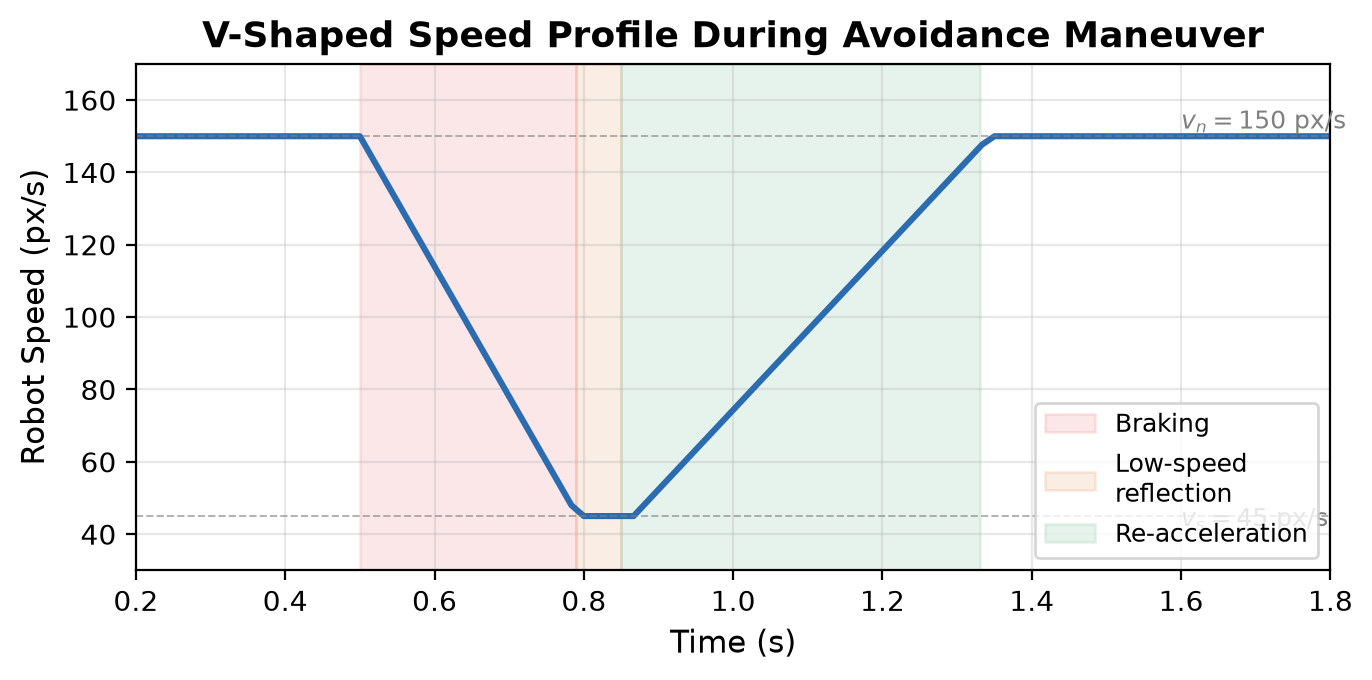
\includegraphics[width=\columnwidth]{speed_profile.png}
\caption{V-shaped speed profile during a single avoidance maneuver. The robot decelerates from $v_n = 150$ px/s to $v_s = 45$ px/s in approximately 0.29 s (braking, red), performs the specular reflection at low speed (orange), and re-accelerates over approximately 0.48 s (green). The rapid deceleration ($a_d = 360$ px/s$^2$) and gradual re-acceleration ($a_a = 220$ px/s$^2$) form an asymmetric profile designed to minimize approach distance while preserving post-maneuver safety margins.}
\label{fig:speed_profile}
\end{figure}

\section{Discussion}

\subsection{Interpretation of Results}

The experimental results validate several design choices. First, the specular reflection mechanism provides a geometrically principled basis for avoidance that the DQN can leverage effectively. Unlike policies that learn arbitrary turning behaviors, the reflection-based approach constrains the action space to physically meaningful maneuvers, improving sample efficiency and producing more predictable trajectories.

Second, the three-phase motion control decomposes the avoidance maneuver into distinct stages, each with clear physical semantics. This decomposition simplifies credit assignment: the policy learns \emph{when} to initiate the sequence, while the \emph{how} of the maneuver is handled by the deterministic physics of deceleration and reflection.

Third, the systematic iteration from V1 through V4 and V3-Shield yields an important negative result: increasing model complexity (V4) and adding external safety rules (V3-Shield) do not necessarily improve performance. V4's additional state variables (braking margin, time-to-collision, circular-path distance) are physically meaningful, yet they alter the state distribution, reward response, and control dynamics in ways that increase the RL search difficulty. V3-Shield's high-frequency forced reflections change the robot's trajectory in ways the original DQN policy was never trained to handle, creating cascade failures near obstacle corners.

\subsection{The Danger of External Safety Patches}

The V3-Shield result deserves particular attention. The Shield was designed as a minimal, conservative safety overlay: it would only intervene when the sensors showed no danger but a geometric path prediction indicated lateral collision risk. In practice, it intervened 4.924 times per episode on average and increased the collision rate from 1.20\% to 6.60\%. The McNemar test ($p \approx 4.63 \times 10^{-7}$) leaves little ambiguity---this is not random fluctuation but a systematic degradation.

This finding has practical implications for the deployment of learned navigation policies. When an already-trained DRL policy is augmented with external rule-based controllers, the coupling between the intervention logic and the policy's learned state distribution must be carefully analyzed. A rule that appears sensible in isolation may, when integrated, push the robot into state regions where the DRL policy has never learned to operate, producing unpredictable and potentially unsafe behavior.

\subsection{Limitations}

Our current approach has several limitations. First, the environment contains only static obstacles; extending to dynamic obstacles would require temporal reasoning about obstacle motion. Second, the discrete action space limits maneuver granularity---a continuous action space could enable finer control over speed and steering. Third, the 2D simulation does not capture the full complexity of real-world robot dynamics, including sensor noise, motor latency, and 3D geometry. Fourth, the training degradation phenomenon observed in V3 and V4 warrants deeper investigation, potentially through analysis of replay buffer dynamics and Q-value distributions over the course of training.

\subsection{Future Work}

Promising directions include: (1) extending the environment to include moving obstacles and multi-agent scenarios; (2) incorporating the MLP collision predictor as an auxiliary input to the DQN state for anticipatory planning; (3) replacing the discrete DQN with continuous-action algorithms such as PPO or SAC for smoother trajectories; (4) deploying the trained policy on a physical robot platform with LiDAR-based sensing; (5) investigating methods to mitigate training degradation, such as periodic policy reset or adaptive exploration schedules; and (6) developing formal verification methods for the coupling between learned policies and external safety rules.

\section{Conclusion}

This paper presented a two-stage framework for robot collision prediction and avoidance that combines supervised learning for collision forecasting with deep reinforcement learning for real-time avoidance control. The key innovation is the integration of a physics-inspired specular reflection mechanism within a three-phase motion control pipeline, which provides a principled geometric basis for avoidance maneuvers while reducing the DRL action space to a binary decision.

Through systematic model iterations and extensive experiments, we draw the following conclusions:

First, an MLP trained on nine-directional sensor readings, linear speed, and angular speed can effectively predict collisions within a 30-frame horizon, achieving 83.65\% accuracy and 84.08\% recall. The multi-directional sensor array captures spatial obstacle distributions that are informative for short-term collision risk assessment.

Second, constraining the DRL action space to two discrete actions---maintain course versus initiate the decelerate-reflect-accelerate sequence---and computing the reflection direction via the specular reflection formula significantly reduces the complexity of the continuous control problem while preserving interpretability.

Third, the design of the reflection normal extraction method and the reward function has a decisive impact on DQN performance. Strictly restricting the normal source to the frontal ray creates perceptual blind spots, while removing the unconditional reflection reward, strengthening the collision penalty, and prioritizing collision rate in model selection substantially improve policy safety.

Fourth, and perhaps most significantly, increasing model complexity and adding external safety rules do not necessarily enhance performance. Both V4 (17-dimensional state with dynamic braking) and V3-Shield (external circular-path collision override) exhibited higher collision rates than V3, due to excessive deceleration, frequent intervention, and unstable normal vectors near obstacle corners. These results caution against the unvalidated layering of safety heuristics onto trained DRL policies.

The final V3 policy achieves a collision rate of 1.20\%, a survival rate of 98.80\%, a mean speed of 148.45 px/s, and a mean episode length of 597.63 steps over 500 independent blind-test episodes, representing a favorable balance between safety and operational efficiency.

\section*{Acknowledgment}
The author thanks the research group for constructive discussions and the open-source community for maintaining the Gymnasium, Stable-Baselines3, and Pygame frameworks that made this work possible.

\begin{thebibliography}{00}

\bibitem{siegwart2011introduction}
R.~Siegwart, I.~R.~Nourbakhsh, and D.~Scaramuzza,
\textit{Introduction to Autonomous Mobile Robots}, 2nd ed.
Cambridge, MA: MIT Press, 2011.

\bibitem{khatib1986real}
O.~Khatib, ``Real-time obstacle avoidance for manipulators and mobile robots,''
\textit{The International Journal of Robotics Research}, vol.~5, no.~1, pp.~90--98, 1986.

\bibitem{borenstein1991vector}
J.~Borenstein and Y.~Koren, ``The vector field histogram---fast obstacle avoidance for mobile robots,''
\textit{IEEE Transactions on Robotics and Automation}, vol.~7, no.~3, pp.~278--288, 1991.

\bibitem{fox1997dynamic}
D.~Fox, W.~Burgard, and S.~Thrun, ``The dynamic window approach to collision avoidance,''
\textit{IEEE Robotics \& Automation Magazine}, vol.~4, no.~1, pp.~23--33, 1997.

\bibitem{ulrich2000vfh}
I.~Ulrich and J.~Borenstein, ``VFH$+$: Reliable obstacle avoidance for fast mobile robots,''
in \textit{Proc. IEEE ICRA}, 2000, pp.~1572--1577.

\bibitem{lavalle2006planning}
S.~M.~LaValle, \textit{Planning Algorithms}.
Cambridge: Cambridge University Press, 2006.

\bibitem{mnih2015human}
V.~Mnih \textit{et al.}, ``Human-level control through deep reinforcement learning,''
\textit{Nature}, vol.~518, no.~7540, pp.~529--533, 2015.

\bibitem{schulman2017proximal}
J.~Schulman, F.~Wolski, P.~Dhariwal, A.~Radford, and O.~Klimov,
``Proximal policy optimization algorithms,''
\textit{arXiv preprint arXiv:1707.06347}, 2017.

\bibitem{haarnoja2018soft}
T.~Haarnoja, A.~Zhou, P.~Abbeel, and S.~Levine,
``Soft actor-critic: Off-policy maximum entropy deep reinforcement learning with a stochastic actor,''
in \textit{Proc. ICML}, 2018, pp.~1861--1870.

\bibitem{lillicrap2015continuous}
T.~P.~Lillicrap \textit{et al.}, ``Continuous control with deep reinforcement learning,''
in \textit{Proc. ICLR}, 2016.

\bibitem{tai2017virtual}
L.~Tai, G.~Paolo, and M.~Liu, ``Virtual-to-real deep reinforcement learning: Continuous control of mobile robots for mapless navigation,''
in \textit{Proc. IEEE/RSJ IROS}, 2017, pp.~31--36.

\bibitem{zhu2017target}
Y.~Zhu \textit{et al.}, ``Target-driven visual navigation in indoor scenes using deep reinforcement learning,''
in \textit{Proc. IEEE ICRA}, 2017, pp.~3357--3364.

\bibitem{kahn2017self}
G.~Kahn, A.~Villaflor, B.~Ding, P.~Abbeel, and S.~Levine,
``Self-supervised deep reinforcement learning with generalized computation graphs for robot navigation,''
in \textit{Proc. IEEE ICRA}, 2018, pp.~5129--5136.

\bibitem{long2018towards}
P.~Long, T.~Fan, X.~Liao, W.~Liu, H.~Zhang, and J.~Pan,
``Towards optimally decentralized multi-robot collision avoidance via deep reinforcement learning,''
in \textit{Proc. IEEE ICRA}, 2018, pp.~6252--6258.

\bibitem{raffin2021stable}
A.~Raffin, A.~Hill, A.~Gleave, A.~Kanervisto, M.~Ernestus, and N.~Dormann,
``Stable-Baselines3: Reliable reinforcement learning implementations,''
\textit{Journal of Machine Learning Research}, vol.~22, no.~268, pp.~1--8, 2021.

\bibitem{towers2023gymnasium}
M.~Towers \textit{et al.}, ``Gymnasium: A standard interface for reinforcement learning environments,''
\textit{arXiv preprint arXiv:2307.13837}, 2023.

\bibitem{van2018deep}
H.~van Hasselt, Y.~Doron, F.~Strub, M.~Hessel, N.~Sonnerat, and J.~Modayil,
``Deep reinforcement learning and the deadly triad,''
\textit{arXiv preprint arXiv:1812.02648}, 2018.

\bibitem{sutton2018reinforcement}
R.~S.~Sutton and A.~G.~Barto,
\textit{Reinforcement Learning: An Introduction}, 2nd ed.
Cambridge, MA: MIT Press, 2018.

\bibitem{goodfellow2016deep}
I.~Goodfellow, Y.~Bengio, and A.~Courville,
\textit{Deep Learning}.
Cambridge, MA: MIT Press, 2016.

\end{thebibliography}

\end{document}
